\subsection{SP7: comunicación y sensado degradados}
\label{sec:resultados-sp7}

\subsubsection{Pregunta y alcance implementado}

SP7 estudia descriptores de red asociados con una campaña de transporte. La conectividad temporal se resume mediante la unión de grafos en una ventana,
\[
 G_{[t-H,t]}=\bigcup_{\tau=t-H}^{t}G(\tau), \qquad
 \lambda_2\!\left(L(G_{[t-H,t]})\right)>0.
\]
Esta condición indica que la información podría propagarse durante la ventana. En la implementación conservada, pérdida, retardo y jitter se aplican al registro de comunicación o se traducen en parámetros agregados; no existe una cola de mensajes que modifique en cada paso el estado vecino usado por un controlador fijo. Por ello, SP7 caracteriza asociación y sensibilidad del modelo, pero no demuestra robustez de transporte en lazo cerrado frente a una red degradada.

\begin{figure}[htbp]
\centering
\resizebox{0.94\textwidth}{!}{%
\begin{tikzpicture}[
  font=\sffamily\small,
  robot/.style={circle,draw=VIUDark!75,fill=VIUOrange!18,line width=0.9pt,minimum size=9mm,font=\sffamily\scriptsize\bfseries},
  memory/.style={draw=VIUDark!65,fill=VIUWhite,rounded corners=3pt,align=center,text width=3.5cm,minimum height=1.2cm,inner sep=5pt},
  flow/.style={-{Latex[length=2.4mm]},line width=0.85pt,draw=VIUDark!70},
  link/.style={line width=0.8pt,draw=VIUOrange!85!black}
]
\node[robot] (r1) at (0,1.4) {$i$};
\node[robot] (r2) at (2.1,2.1) {$j$};
\node[robot] (r3) at (2.1,0.7) {$h$};
\node[robot] (r4) at (4.2,1.4) {$\ell$};
\draw[link] (r1)--(r2)--(r4)--(r3)--(r1);
\draw[link,dashed] (r2)--(r3);
\node[font=\scriptsize,align=center] at (2.1,-0.05) {grafo local $G(t)$\\con p\'erdidas y retardos};

\node[memory] (mem) at (7.2,1.4) {Memoria local\\descriptores, ocupaci\'on y antig\"uedad};
\node[memory] (decision) at (11.4,1.4) {Decisi\'on distribuida\\coalici\'on y rel\'e};
\node[memory] (check) at (11.4,-1.1) {Comprobaci\'on temporal\\$\lambda_2(\cup_\tau G(\tau))>0$};

\draw[flow] (r4) -- (mem);
\draw[flow] (mem) -- (decision);
\draw[flow] (decision) -- (check);
\draw[flow] (check.west) -| (mem.south);
\end{tikzpicture}}
\caption[Flujo de informaci\'on bajo comunicaci\'on degradada]{Flujo de informaci\'on considerado en SP7. Las decisiones usan memoria local y conectividad acumulada en una ventana temporal; no presuponen una vista global instant\'anea de la flota.}
\viuownsource
\label{fig:sp7-information-flow}
\end{figure}


\subsubsection{Métodos y diseño experimental}

\begin{table}[H]
\centering
\scriptsize
\begin{tabularx}{\textwidth}{@{}p{0.31\textwidth}p{0.18\textwidth}X@{}}
\toprule
Método & Alcance & Función en SP7 \\
\midrule
Referencia con comunicación completa & Centralizado & Comparador interno con estado global. \\
Control global clásico & Proxy centralizado & Dependencia de información agregada. \\
APF con sensores locales & Descentralizado & Comparador reactivo de baja comunicación. \\
Consenso tolerante a retardos & Proxy adaptado & Sensibilidad paramétrica a mensajes vecinos. \\
CBF conectado y CBBA con relés & Proxies mixtos & Seguridad y subasta bajo descriptores de red. \\
Reparación local robusta al retardo & Descentralizado & Selección de relés y reparación por eventos. \\
Juego \emph{wrench} sensible a conectividad & Descentralizado & Variante con precios físicos y de enlace. \\
\bottomrule
\end{tabularx}
\caption{Métodos representativos y alcance de implementación en SP7.}
\label{tab:sp7-methods}
\end{table}

La campaña combina seis familias de escenarios, cinco perfiles y 97 semillas. Los ocho métodos generan $20\,176$ filas. Estas filas repiten mundos por método y perfil; por tanto, no representan $20\,176$ observaciones independientes. La unidad para una inferencia válida es el mundo o bloque completo de mundo y perfil.

\subsubsection{Resultados descriptivos}

\begin{figure}[H]
\centering
\begin{minipage}[t]{0.49\textwidth}
\centering
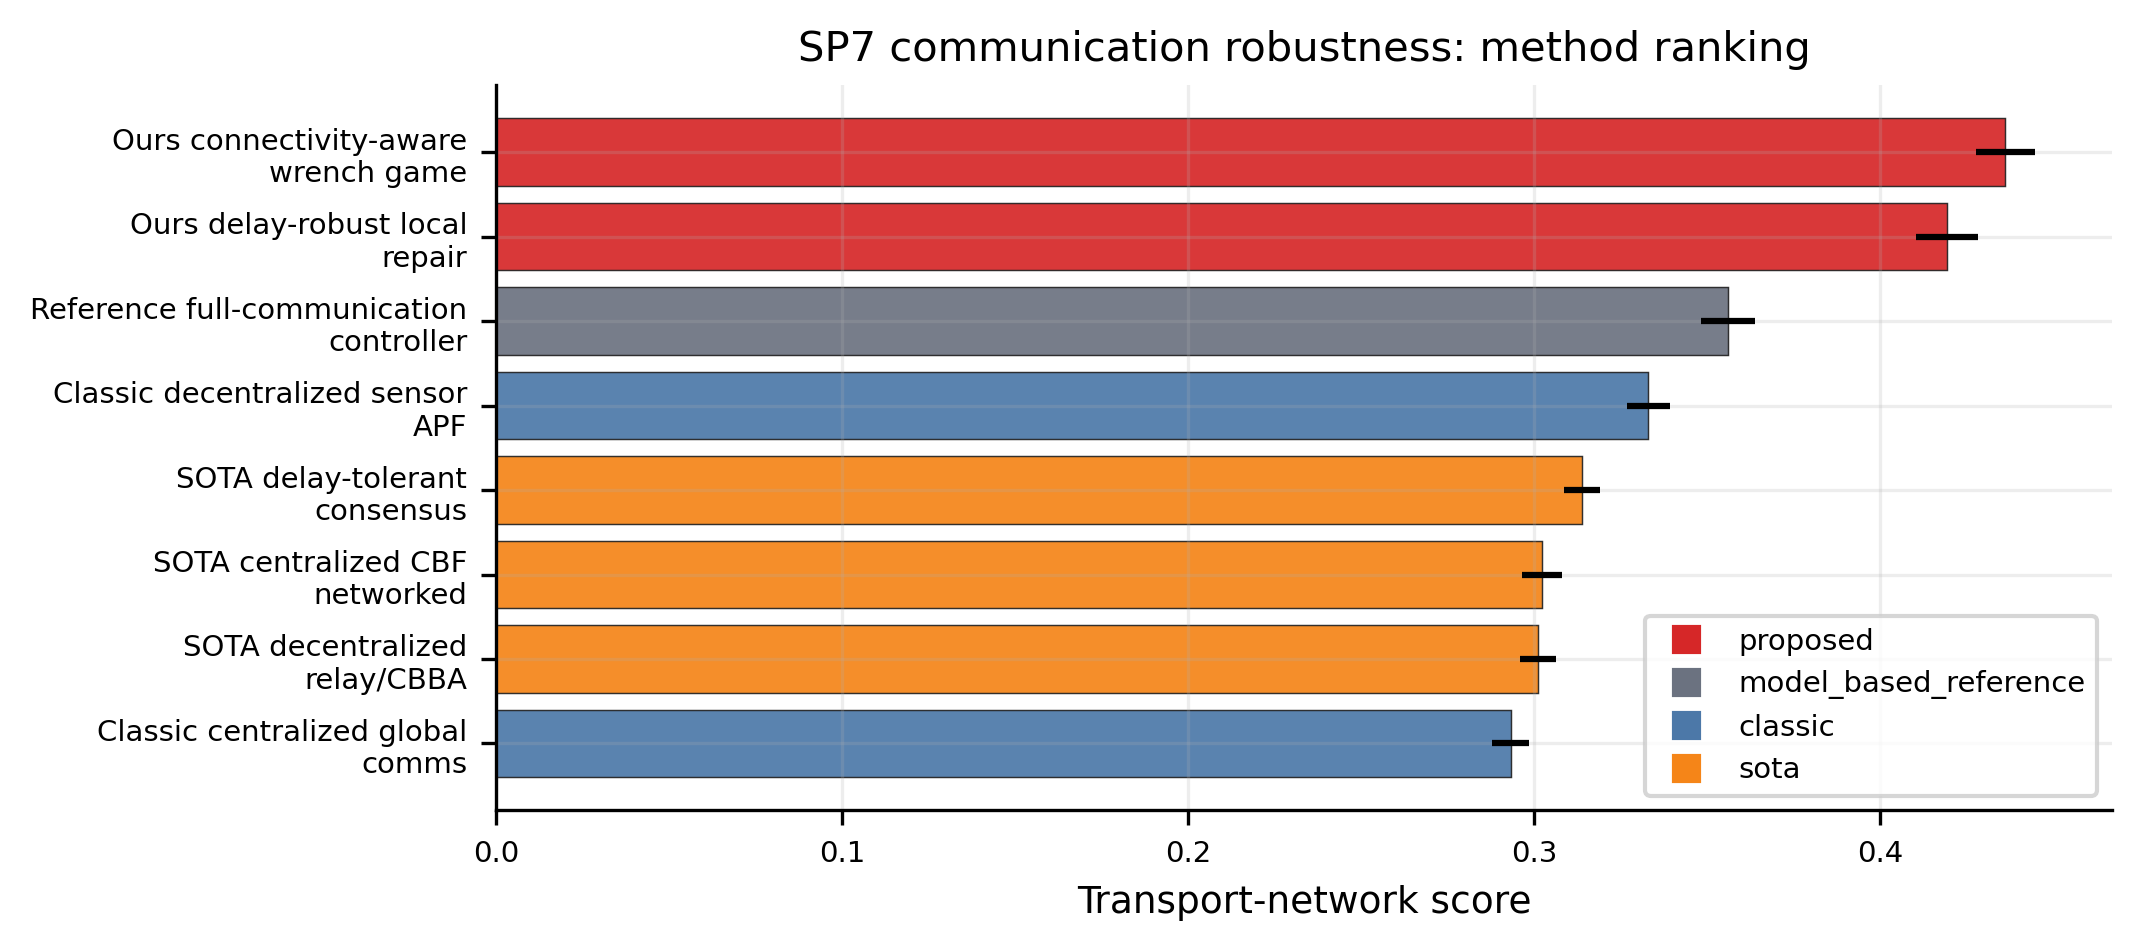
\includegraphics[width=\linewidth]{figures/fig-sp7-primary.png}
\end{minipage}\hfill
\begin{minipage}[t]{0.49\textwidth}
\centering
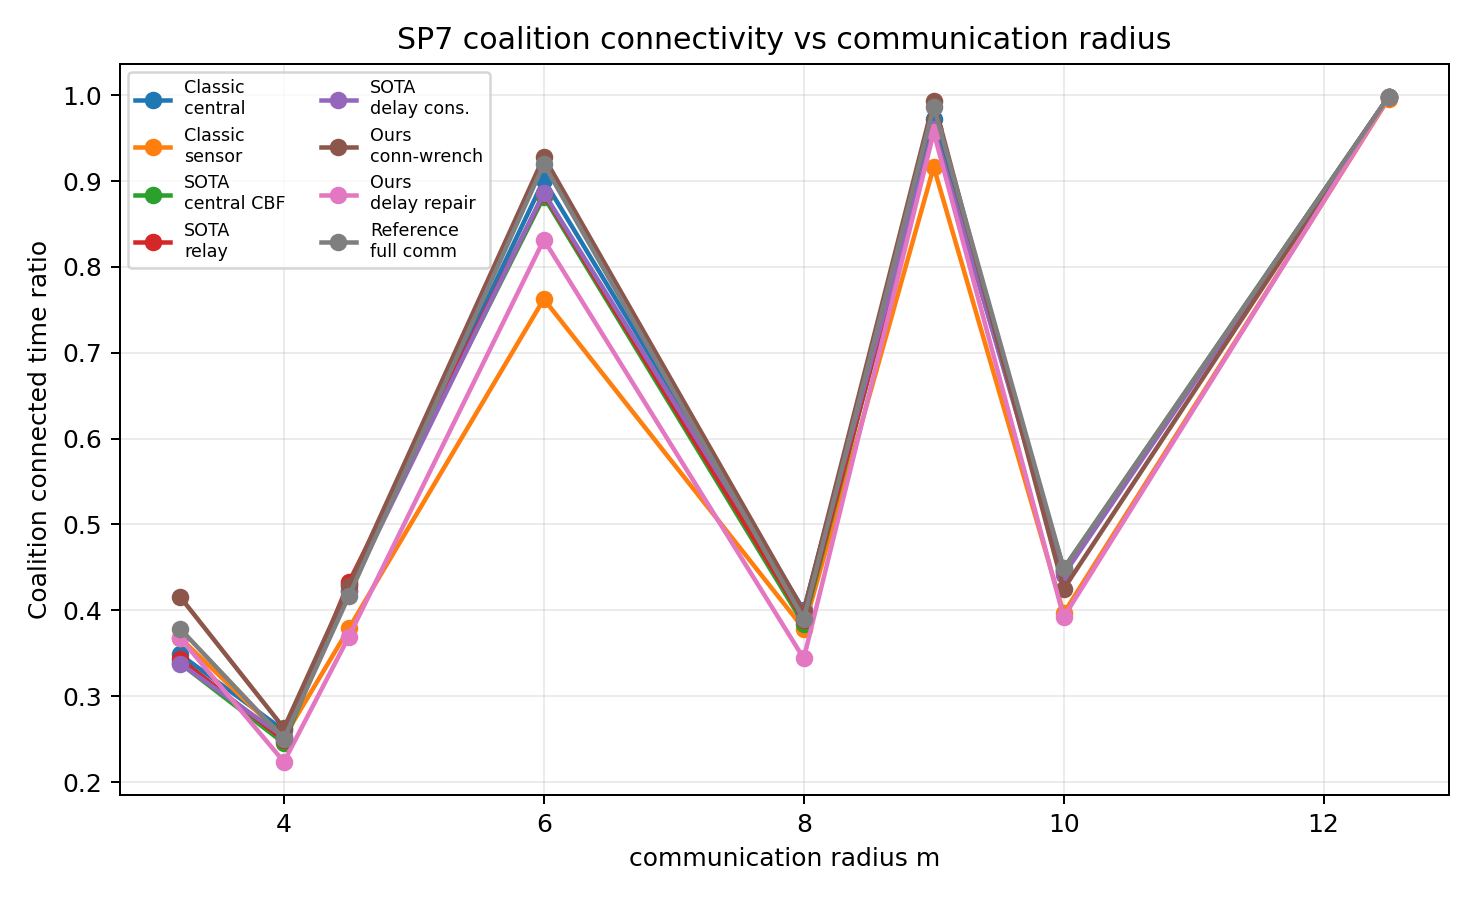
\includegraphics[width=\linewidth]{figures/fig-sp7-connectivity.png}
\end{minipage}
\caption[Resultados descriptivos de SP7]{Rendimiento agregado y conectividad en función del radio de comunicación. Las asociaciones no equivalen a efectos causales de un canal dentro del lazo.}
\viuownsource
\label{fig:sp7-primary}
\label{fig:sp7-connectivity}
\end{figure}

El juego \emph{wrench} sensible a conectividad registra $0{,}1423$ de transporte, $0{,}3096$ de éxito de relé y $0{,}9100$ de conectividad temporal. La reparación robusta conserva la misma tasa de transporte y registra $0{,}2354$ de relé. La referencia de comunicación completa alcanza $0{,}0777$ de transporte y $0{,}3181$ de relé. CBBA con relés y el control global clásico obtienen $0{,}0206$ y $0{,}0214$ de transporte, respectivamente. Estas diferencias describen la campaña implementada; las funciones de control no son idénticas y la referencia global no constituye una cota uniforme.

La correlación fila a fila entre radio y conectividad es $\rho=0{,}8934$. Se conserva como diagnóstico descriptivo porque el cálculo repite mundos entre tratamientos. El contraste H7.3 de intermitencia extrema no dispone de bloques completos ($n_{\rm bloques}=0$) y, por tanto, es \textbf{no estimable}. El valor heredado $p=1$ no se interpreta como ausencia de diferencias.

\subsubsection{Límite y trabajo necesario}

Una prueba confirmatoria de H7 requiere mantener fijo el controlador e introducir dentro de cada paso colas de mensajes, timestamps, pérdida, retardo, estados vecinos obsoletos y expiración de memoria. El análisis debe agrupar por mundo y reportar efecto, intervalo, número efectivo de clusters y eventos. Hasta entonces, SP7 respalda únicamente la utilidad descriptiva de medir conectividad temporal; no prueba tolerancia cerrada a intermitencia extrema.
